\begin{surferPage}[منحنى كومر المربع]{منحنى كومر المربع}
    في العام 1875، كان إدوارد كومر %
\textenglish{(Eduard Kummer)} %
      أول من تساءل مباشرة عن العدد الأقصى $\mu(d)$ لمتفردات منحنيات من الدرجة $d$، في حال منحنيات من الدرجة $4$ والمسماة \emph{منحنيات مربعة }.

  لقد أثبت أن $\mu(4)=16$. بعدها، إنصرف إلى دراسة المنحنيات المربعة ذات $16$ متفرداً.
   عائلة جميلة من هذه السطوح معطاة بواسطة المعادلات:
    \[\bigl(x^2+y^2+z^2-\mu^2\bigr)^2 - \lambda
    \,y_0\,y_1\,y_2\,y_3,\]
    حيث $\mu$ بارامتر حر وحيث
    $\lambda = \frac{3\mu^2-1}{3-\mu^2}$;
وحيث $y_i$ هي أضلاع رباعي سطوح منتظم {\small
    $y_0=1-z-\sqrt{2}x$, \
    $y_1=1-z+\sqrt{2}x$, \
    $y_2=1+z+\sqrt{2}y$, \
    $y_3=1+z-\sqrt{2}y$}
 السطح متناظراً.
  لا يملك كل أعضاء هذه العائلة $16$ متفرداً حقيقياً بالضبط، ولكن معظمهم:
  \begin{center}
    \vspace*{-0.2cm}\hspace*{-0.2cm}
    \begin{tabular}{@{}c@{\,}c@{\,}c@{\,}c@{\,}c@{}}
      \begin{tabular}{@{}c@{}}
        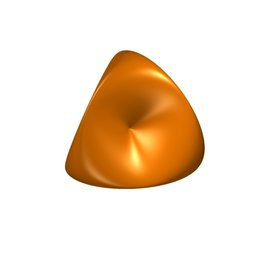
\includegraphics[height=1.4cm]{kummer_0}
      \end{tabular}
      &
      \begin{tabular}{@{}c@{}}
        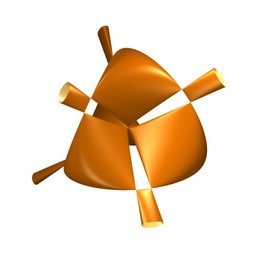
\includegraphics[height=1.4cm]{kummer_1}
      \end{tabular}
      &
      \begin{tabular}{@{}c@{}}
        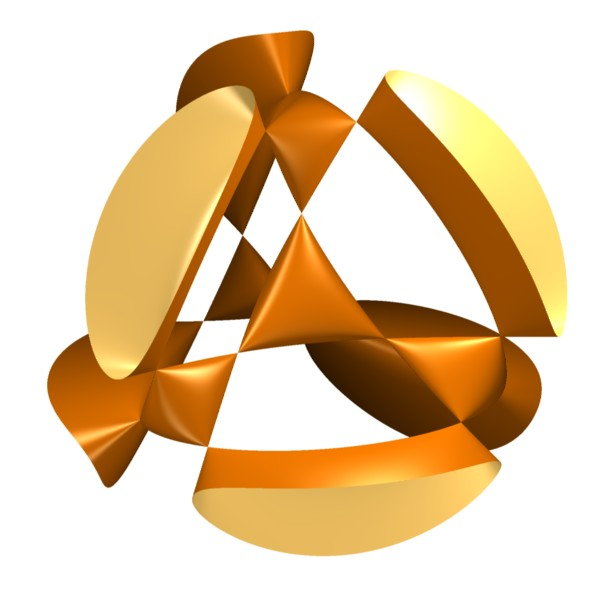
\includegraphics[height=1.4cm]{kummer_2}
      \end{tabular}
      &
      \begin{tabular}{@{}c@{}}
        
\includegraphics[height=1.4cm]{kummer_3}
      \end{tabular}
    \end{tabular}
  \end{center}
  \vspace{-0.2cm}
  لبعض قيم خاصة نعطيها للبارامترات، يحدث أن تتطابق عدة من المتفرادات.
\end{surferPage}
